\section{Monte Carlo Simulation of Liquid Argon}

The Monte Carlo method can be used to simulate argon liquid, at a given temperature, through
the canonical ensemble. The results of a canonical simulation should agree very closely with
the results of a microcanonical simulation (molecular dynamics), differing only due to the
fact that the number of particles, while large, is not infinite.

Your molecular dynamics code can be easily modified to do a Monte Carlo simulation by
replacing the Verlet algorithm part of the code with a Metropolis update for each particle
and velocity. Of course, you do not need to do the velocity via Monte Carlo, since it is a
Maxwell distribution, but it is a negligible computational overhead to include it and it
keeps the changes in your code small.

\Question{}
Modify your argon molecular dynamics code to do a Monte Carlo simulation at a temperature of
\(T = 1.069\) and density \(\rho = 0.75\). Measure the same variables as in Problem Set 2
and check that your answers agree. Include statistical errors for your results.

\Answer{}
For the Monte Carlo (MC) calculations, there is no objective definition of time. The notion
of time is replaced with \emph{sweeps}. For an \(N\)-particle system, one MC sweep
corresponds to \(N\) attempts of displacement of particle positions, where the Metropolis
algorithm is employed to decide the acceptance of an atomic displacement. In each attempt,
one randomly selected atom \(i\) is displaced in each Cartesian direction
\(\alpha\) by
%
\begin{equation}\label{eq:ri}
    r_{i, \alpha}' = r_{i, \alpha} + \delta (\code{rand()} - 0.5),
\end{equation}
%
where \(i = 1\), \(2\), \(\ldots\), \(N\), and \(\alpha = 1\), \(2\), \(3\),
and \(r_{i, \alpha}'\) is the new trial position of the particle in the next time step,
and \(\delta\) is a parameter that controls the maximum size of displacements (amplitude)
and \code{rand()} is a function that will generate a
uniformly distributed random number between \(0\) and \(1\).
So, in each trial move, we are going to update the position of the particle
by a random number between \(-0.5\) and \(0.5\) in each Cartesian direction.
This is because to satisfy the detailed balance condition, we need an equal chance
of moving forward and backward.

The value of \(\delta\) is a key
ingredient of the MC simulation. If it is too large, there follows a high probability
for the resulting configuration to have high energy, and thus the trial move has a
large probability of being rejected.
In this case, we are wasting a lot of time on each sweep.
On the other hand, if \(\delta\) is too small, the change in
potential energy is also small so that most trials will be accepted, but the configuration
space would be sampled poorly since we are not moving too far.
For all simulations (unless stated otherwise), the
value of \(\delta\) is adjusted after each sweep so as to get an acceptance ratio (number of
accepted attempts over the total number of attempts) of approximately \(0.5\).

A more sophisticated solution is also to update the velocity of the particle
at the same time as we update its position. So that we could keep the concept of
``time step'' and wrap it in the same application programming interface (API)
as the Verlet algorithm.
That is, rewrite Equation~\eqref{eq:ri} as
%
\begin{align}
    v_{i, \alpha}' & = v_{i, \alpha} + \delta (\code{rand()} - 0.5),\label{eq:vnew} \\
    r_{i, \alpha}' & = r_{i, \alpha} + v_{i, \alpha}' \Delta t,\label{eq:rnew}
\end{align}
%
where \(\Delta t\) is the width of each time step.
However, we need to be careful when adjusting these parameters (i.e., \(\delta\) and
\(\Delta t\)). The change in total energy is now
%
\begin{align}
    \Delta U & = U' - U = \frac{1}{2} = \sum_{\substack{i, j                            \\ j \neq i}} \bigl(u'(r_{ij}) - u(r_{ij})\bigr),\label{eq:dU} \\
    \Delta K & = K' - K = \frac{1}{2} m \bigl(v_{i, \alpha}'^2 - v_{i, \alpha}^2\bigr),
\end{align}
%
note that the change in the potential energy is much more complicated than that of the
kinetic energy since when we update the position of one particle, the distances
between it and all the rest particles have changed.
In the~\eqref{eq:ri} case, only~\eqref{eq:dU} is considered.
So, if \(\delta\) and \(\Delta t\) are not tuned, we could result in one trial move.
Then the difference between \(\Delta U\) and \(\Delta K\) will be huge, resulting in a
biased change in total energy and a low acceptance ratio.

However, this solution is too tricky, so we do not adopt it here.
What we used is a more flexible solution, that is, adjusting position and velocity
with two independent parameters. Rewrite Equations~\eqref{eq:vnew} and~\eqref{eq:rnew} as
%
\begin{align}
    v_{i, \alpha}' & = v_{i, \alpha} + \delta_v (\code{rand()} - 0.5), \\
    r_{i, \alpha}' & = r_{i, \alpha} + \delta_r (\code{rand()} - 0.5),
\end{align}
%
where the two parameters \(\delta_v\) and \(\delta_r\) are controlled by us according to
the simulation process. The complete algorithm adopted is listed in
Snippet~\ref{lst:take_one_step}.
%
\begin{algorithm}[H]
    \caption{The Metropolis--Hastings algorithm for sampling the phase space in a canonical
        ensemble of the liquid argon system.}
    \label{lst:take_one_step}
    \begin{juliacode}
        function take_one_step!(particles, box::Box, δv, δr, integrator::MetropolisHastings)
            for (i, particle) in enumerate(particles)
                r = rand(3) .- 0.5  # Random numbers from -0.5 to 0.5
                velocity = particle.velocity .+ δv .* r
                coordinates = particle.coordinates .+ δr .* r
                map!(Base.Fix2(mod, box.side_length), coordinates, coordinates)
                new_particle = Particle(coordinates, velocity)
                new_particles = map(enumerate(particles)) do (j, old_particle)
                    j == i ? new_particle : old_particle
                end
                ΔU = potential_energy(new_particles) - potential_energy(particles)
                ΔK = kinetic_energy(new_particle) - kinetic_energy(particle)
                ΔE = ΔU + ΔK
                P = exp(-integrator.β * ΔE)
                if P > rand()
                    particles[i] = new_particle
                end
            end
            return particles
        end
    \end{juliacode}
\end{algorithm}
%
Of course, in this simulation, we still need to apply the periodic boundary conditions.
And in reality, we also have a few lines of code to check the acceptance ratio to be
around \(0.5\).

So how to choose \(\delta_r\) and \(\delta_v\)? One way is to check how large
a stride was in our Verlet molecular dynamics simulation and set comparable values
for them.

With that in mind, we plot the simulation for \(3805\) steps with each time step (even
though it is not actually used) as \(0.02\), as shown in Figure~\ref{fig:mcmd}.
The initial values of \(\delta_v\) and \(\delta_r\) are \(0.5\) and \(0.05\),
respectively. We changed \(\delta_v\) and \(\delta_r\) in the latter part of the
simulation (around \(t = 60\) and \(t = 65\)) to approximate to better results.
As we can see, after \(1000\) steps, the system is well-thermalized.
%
\begin{figure}
    \centering
    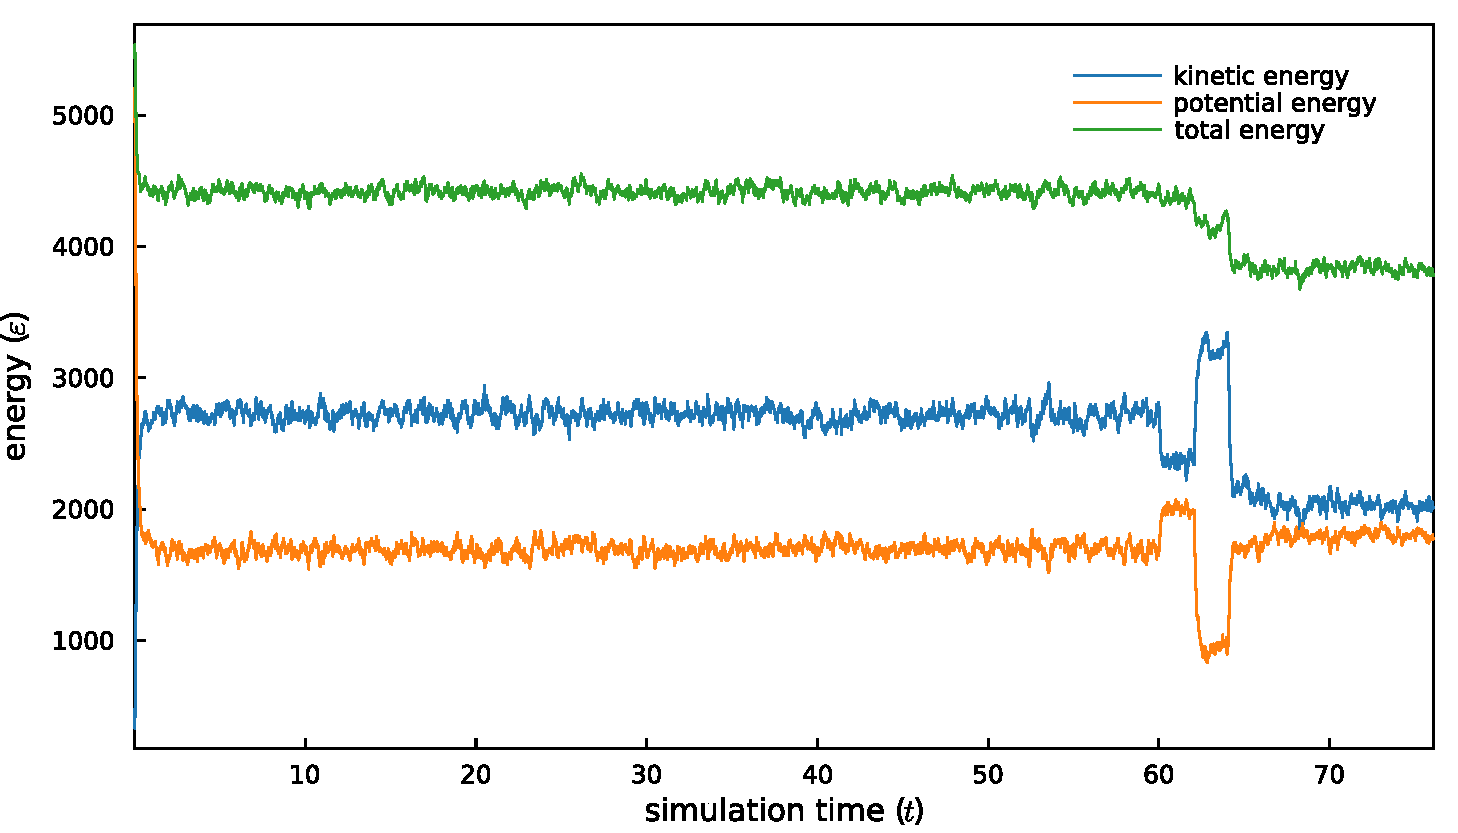
\includegraphics[width=0.9\textwidth]{mcmd}
    \caption{The potential, kinetic, and total energies of a Monte Carlo simulation of
        liquid argon using the Metropolis--Hastings algorithm.
        The initial values of \(\delta_v\) and \(\delta_r\) are \(0.5\) and \(0.05\),
        respectively. We changed \(\delta_v\) and \(\delta_r\) in the latter part of the
        simulation (around \(t = 60\) and \(t = 65\)) to approximate to better results.}
    \label{fig:mcmd}
\end{figure}
%
And the temperature during this simulation is plotted in Figure~\ref{fig:mc_T}.
However, as stated, we did not converge to a value of around \(T = 1.073\), but
around \(2.10\) (considering only steps from \(1000\) to \(3000\)).
We will use this data in the following text as the foundation of our analysis.
The estimated pressure is \(\beta P / \rho \approx 0.16345\), not \(1.0004\)
as in Problem Set 2.

\begin{figure}
    \centering
    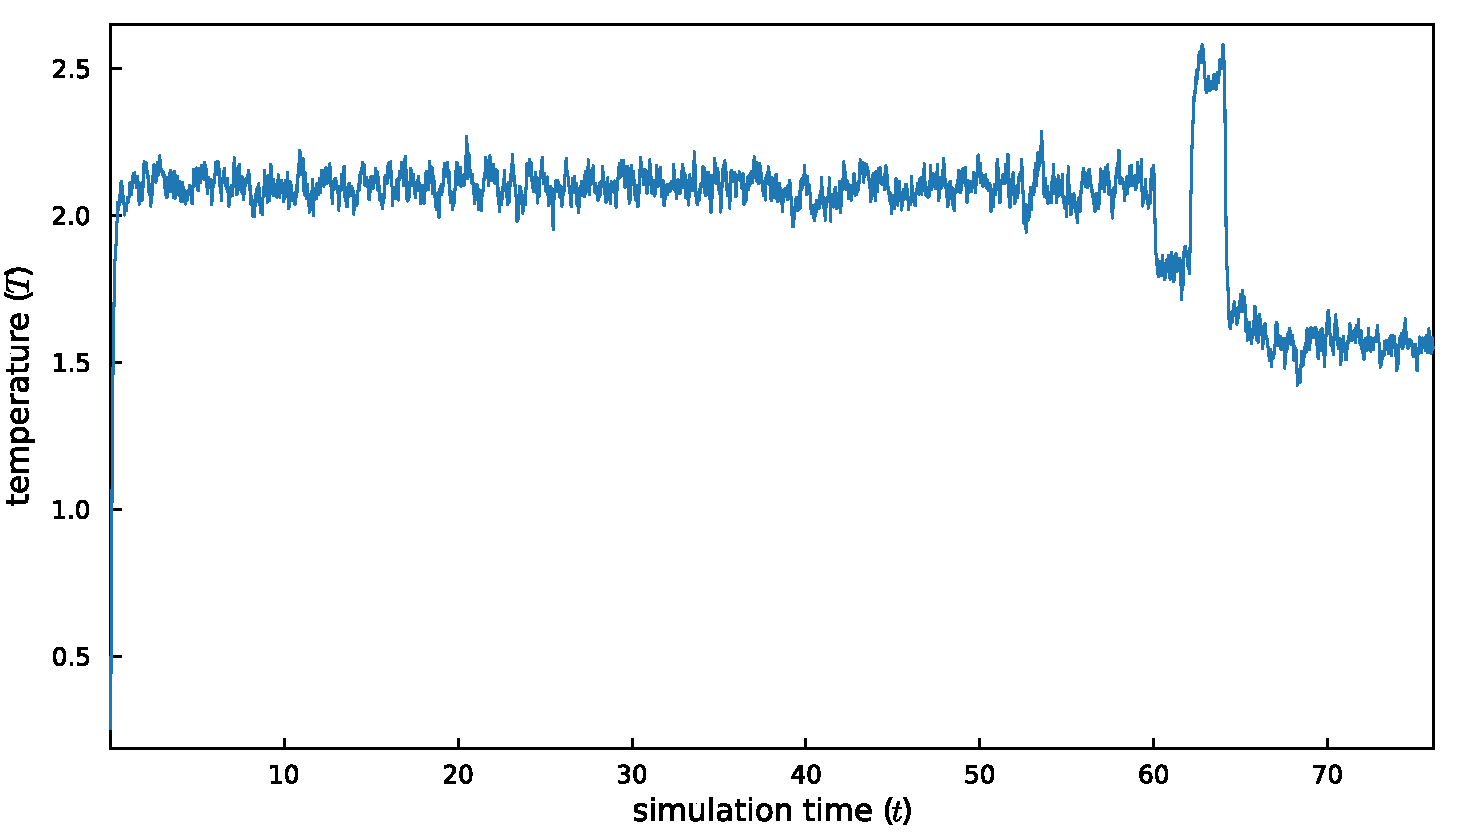
\includegraphics[width=0.9\textwidth]{mc_T}
    \caption{The temperature of a Monte Carlo simulation of
        liquid argon using the Metropolis--Hastings algorithm.
        We will only use the data from \(t = 20\) (the \(1000\)th step)
        to \(t = 60\) (the \(3000\)th step) in the following analysis.}
    \label{fig:mc_T}
\end{figure}

\Question{}
In the molecular dynamics simulations, the autocorrelation times for observables are related
to physical quantities, since the evolution represents the real dynamics of the system. For
the Monte Carlo, the autocorrelation time reflects the algorithm used for the update. Quote
measured integrated autocorrelation time for the measured temperature.

\Answer{}
The integrated autocorrelation time for the measured temperature is plotted in
Figure~\ref{fig:MD_tau_temperature}.

\begin{figure}
    \centering
    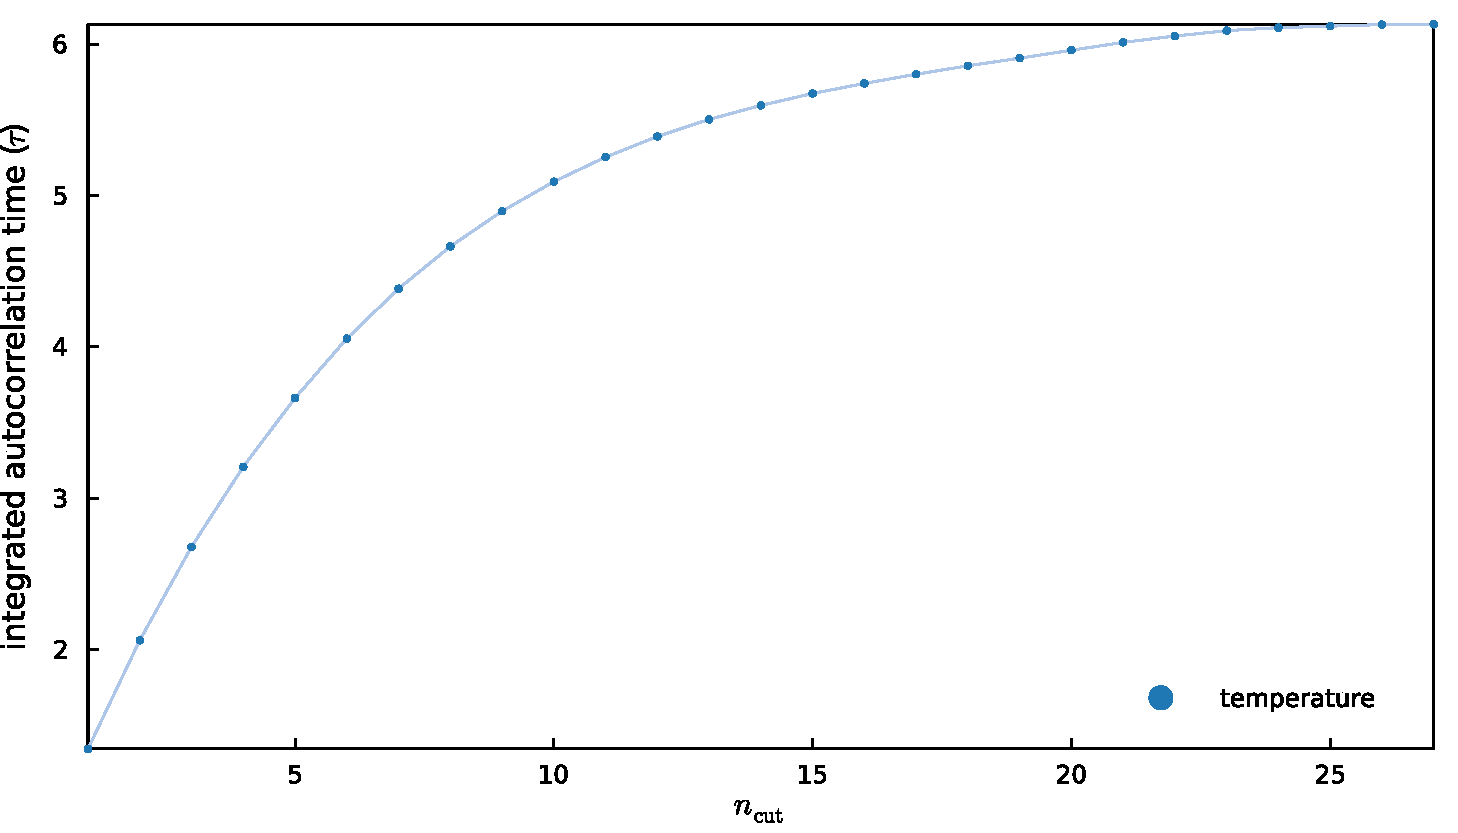
\includegraphics[width=0.9\textwidth]{MD_tau_temperature}
    \caption{The integrated autocorrelation time for the measured temperature
        in our Monte Carlo simulation.}
    \label{fig:MD_tau_temperature}
\end{figure}

Since we only select \(2000\) steps, the integrated autocorrelation time
cannot be too large.
The integrated autocorrelation time for the potential energy, kinetic energy,
and total energy are plotted in Figure~\ref{fig:MD_tau_energy}.

\begin{figure}
    \centering
    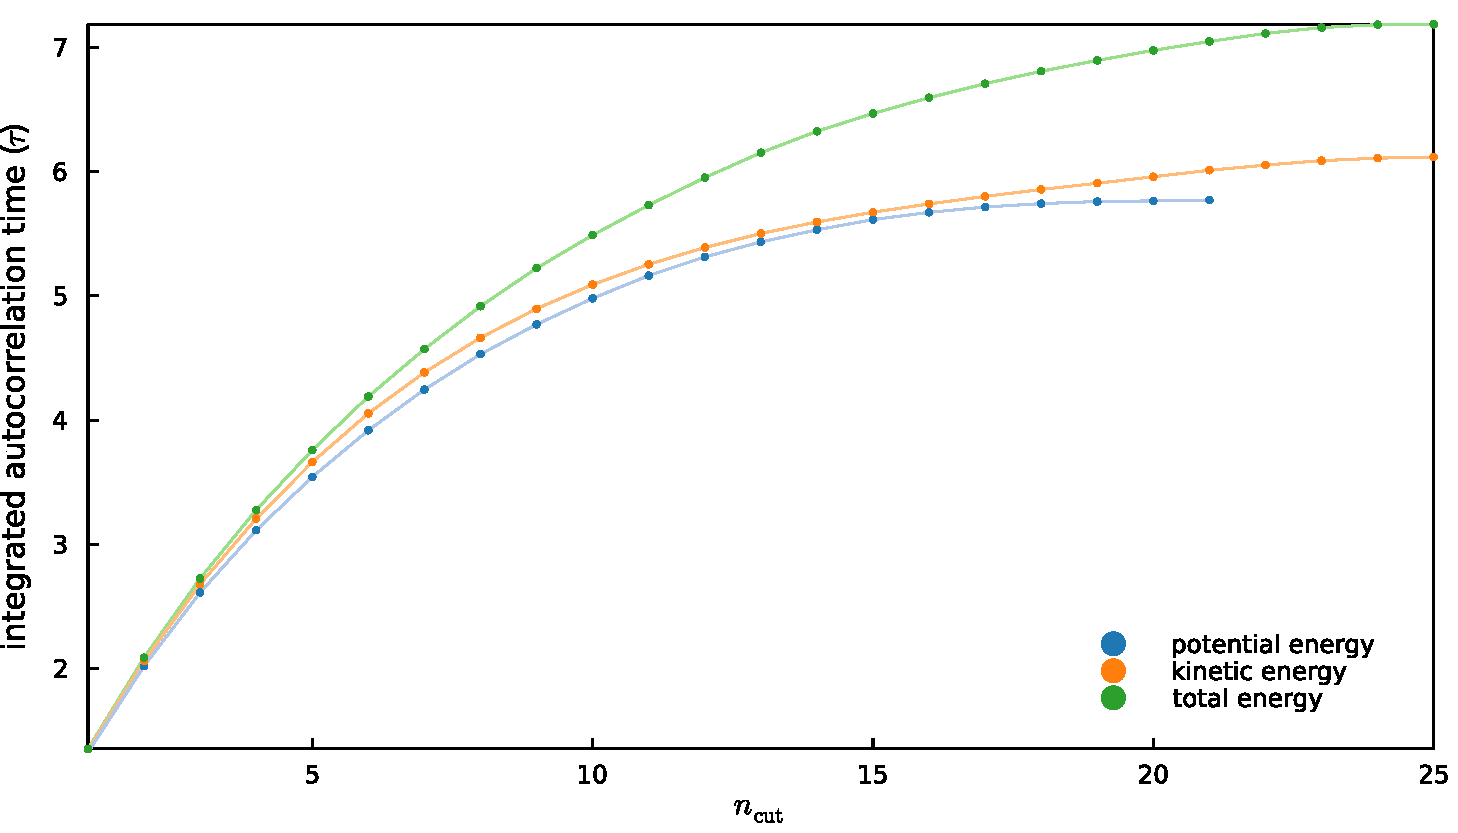
\includegraphics[width=0.9\textwidth]{MD_tau_energy}
    \caption{The integrated autocorrelation time for the potential energy, kinetic energy,
        and total energy.}
    \label{fig:MD_tau_energy}
\end{figure}
